\documentclass[11pt, a4paper]{article}
\usepackage{graphicx}
\usepackage{geometry} % Necessary package for defining margins

\geometry{
	top=1cm, % Defines top margin
	bottom=2cm, % Defines bottom margin
	left=2.2cm, % Defines left margin
	right=2.2cm, % Defines right margin
	includehead, % Includes space for a header
	%includefoot, % Includes space for a footer
	%showframe, % Uncomment if you want to show how it looks on the page 
}

\setlength{\parindent}{15pt}

%---------------------------------------------------------------------------------
% Define your spacing
\usepackage{setspace} % Required for spacing
% Two options:
\linespread{1}
%\onehalfspacing % one-half-spacing linespread
%----------------------------------------------------------------------------------------
% Define your fonts
\usepackage[T1]{fontenc} % Output font encoding for international characters
\usepackage[utf8]{inputenc} % Required for inputting international characters

\usepackage{hyperref}
\hypersetup{
  colorlinks   = true, %Colours links instead of ugly boxes
  urlcolor     = blue, %Colour for external hyperlinks
  linkcolor    = blue, %Colour of internal links
  citecolor   = red %Colour of citations
}

\usepackage{parskip}
\usepackage{listings}
\usepackage{color}
\definecolor{lightgray}{gray}{0.9}

\lstset{
    showstringspaces=false,
    basicstyle=\ttfamily,
    keywordstyle=\color{blue},
    commentstyle=\color[grey]{0.6},
    stringstyle=\color[RGB]{255,150,75}
}

\newcommand{\inlinecode}[2]{\colorbox{lightgray}{\lstinline[language=#1]$#2$}}


%---------------------------------------------------------------------------------
% Define your headers and footers

\usepackage{fancyhdr} % Package is needed to define header and footer
\pagestyle{fancy} % Allows you to customize the headers and footers

%\renewcommand{\sectionmark}[1]{\markboth{#1}{}} % Removes the section number from the header when \leftmark is used

% Headers
\lhead{} % Define left header
\chead{\textit{}} % Define center header - e.g. add your paper title
\rhead{} % Define right header

% Footers
\lfoot{} % Define left footer
\cfoot{\footnotesize \thepage} % Define center footer
\rfoot{ } % Define right footer

%---------------------------------------------------------------------------------
%	Add information on bibliography
\usepackage{natbib} % Use natbib for citing

% For citing with natbib, you may want to use this reference sheet: 
% http://merkel.texture.rocks/Latex/natbib.php

%---------------------------------------------------------------------------------
% Add field for signature (Reference: https://tex.stackexchange.com/questions/35942/how-to-create-a-signature-date-page)
\newcommand{\signature}[2][5cm]{%
  \begin{tabular}{@{}p{#1}@{}}
    #2 \\[2\normalbaselineskip] \hrule \\[0pt]
    {\small \textit{Signature}} \\[2\normalbaselineskip] \hrule \\[0pt]
    {\small \textit{Place, Date}}
  \end{tabular}
}


\title{Python Mini Tutorial}
\date{ 9 Juli 2019}
\author{Mula Cloud Project}
 
\begin{document}

\pagenumbering{gobble}
\maketitle
\newpage

\tableofcontents
\newpage
\pagenumbering{arabic}

\setcounter{page}{1}
\section{Pengenalan}
\subsection{Apa itu Python}
Python adalah bahasa pemrograman interpretatif multiguna dengan filosofi perancangan yang berfokus pada tingkat keterbacaan kode. Python diklaim sebagai bahasa yang menggabungkan kapabilitas, kemampuan, dengan sintaksis kode yang sangat jelas, dan dilengkapi dengan fungsionalitas pustaka standar yang besar serta komprehensif. Python juga didukung oleh komunitas yang besar

\subsection{Sejarah}
Python dikembangkan oleh Guido van Rossum pada tahun 1990 di Stichting Mathematisch Centrum (CWI), Amsterdam sebagai kelanjutan dari bahasa pemrograman ABC. Versi terakhir yang dikeluarkan CWI adalah 1.2

\subsection{Fitur}

\begin{itemize}
    \item Memiliki kepustakaan yang luas; dalam distribusi Python telah disediakan modul-modul 'siap pakai' untuk berbagai keperluan.
    \item Memiliki tata bahasa yang jernih dan mudah dipelajari.
    \item Memiliki aturan layout kode sumber yang memudahkan pengecekan, pembacaan kembali dan penulisan ulang kode sumber.
    \item Berorientasi objek.
    \item Memiliki sistem pengelolaan memori otomatis (garbage collection, seperti java)
    \item Modular, mudah dikembangkan dengan menciptakan modul-modul baru; modul-modul tersebut dapat dibangun dengan bahasa Python maupun C/C++.
    \item Memiliki fasilitas pengumpulan sampah otomatis, seperti halnya pada bahasa pemrograman Java, python memiliki fasilitas pengaturan penggunaan ingatan komputer sehingga para pemrogram tidak perlu melakukan pengaturan ingatan komputer secara langsung.
    \item Memiliki banyak faslitas pendukung sehingga mudah dalam pengoperasiannya.
\end{itemize}

\subsection{Dimana digunakan ?}
Penggunaan python saat ini sudah sangat meluas. Berbagai perusahaan IT terkemuka sudah menggunakannya seperti:
\begin{itemize}
    \item  Google
    \item  Bitbucket
    \item  Youtube
    \item  Instagram
    \item  NASA
    \item  Pintarest
\end{itemize}
\newpage 


\section{Instalasi Python}
Saat ini terdapat dua versi python yang masih beredar yaitu versi 2.x dan versi 3.x.
Namun begitu pada tutorial ini kita hanya akan menggunakan versi 3.x. Hal ini dikarenakan
versi 2.x akan berhenti supportnya pada tahun 2020.

Langkah awal untuk installasi adalah mengunduh file instalasi Python di \url{https://www.python.org/downloads/windows/}.

Untuk versi Windows 32bit silahkan unduh versi Python yang x86 sedangkan untuk yang 62bit silahkan unduh yang x86\_64

Setelah file instalasi terunduh maka silahkan eksekusi file tersebut kemudian ikut instruksi di dalamnya.

Apabila instalasi telah berjalan dengan baik dan benar maka kita dapat memanggil Python dari CMD Windows. 

Ketikan \inlinecode{Java}{python} di CMD masing - masing, perintah ini akan memanggil Read Eval Print Loop ( REPL ) dari Python.
Di sini kita bisa mengetikan perintah untuk kemudian di eksekusi oleh Python. Akan muncul seperti gambar di bawah ini
\begin{figure}[h]
\begin{center}
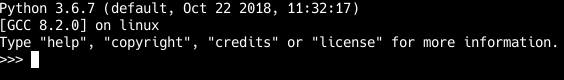
\includegraphics[width=0.8\linewidth]{img/python}
\caption{Python REPL}
\end{center}
\end{figure}
\newpage

\input{coba}
\section{Instalasi Python}
Saat ini terdapat dua versi python yang masih beredar yaitu versi 2.x dan versi 3.x.
Namun begitu pada tutorial ini kita hanya akan menggunakan versi 3.x. Hal ini dikarenakan
versi 2.x akan berhenti supportnya pada tahun 2020.

Langkah awal untuk installasi adalah mengunduh file instalasi Python di \url{https://www.python.org/downloads/windows/}.

Untuk versi Windows 32bit silahkan unduh versi Python yang x86 sedangkan untuk yang 62bit silahkan unduh yang x86\_64

Setelah file instalasi terunduh maka silahkan eksekusi file tersebut kemudian ikut instruksi di dalamnya.

Apabila instalasi telah berjalan dengan baik dan benar maka kita dapat memanggil Python dari CMD Windows. 

Ketikan \inlinecode{Java}{python} di CMD masing - masing, perintah ini akan memanggil Read Eval Print Loop ( REPL ) dari Python.
Di sini kita bisa mengetikan perintah untuk kemudian di eksekusi oleh Python. Akan muncul seperti gambar di bawah ini
\begin{figure}[h]
\begin{center}
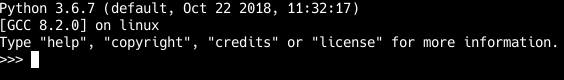
\includegraphics[width=0.8\linewidth]{img/python}
\caption{Python REPL}
\end{center}
\end{figure}
\newpage


\end{document}
